\documentclass{standalone}
\usepackage{tikz}
\usepackage{amsmath}
\begin{document}

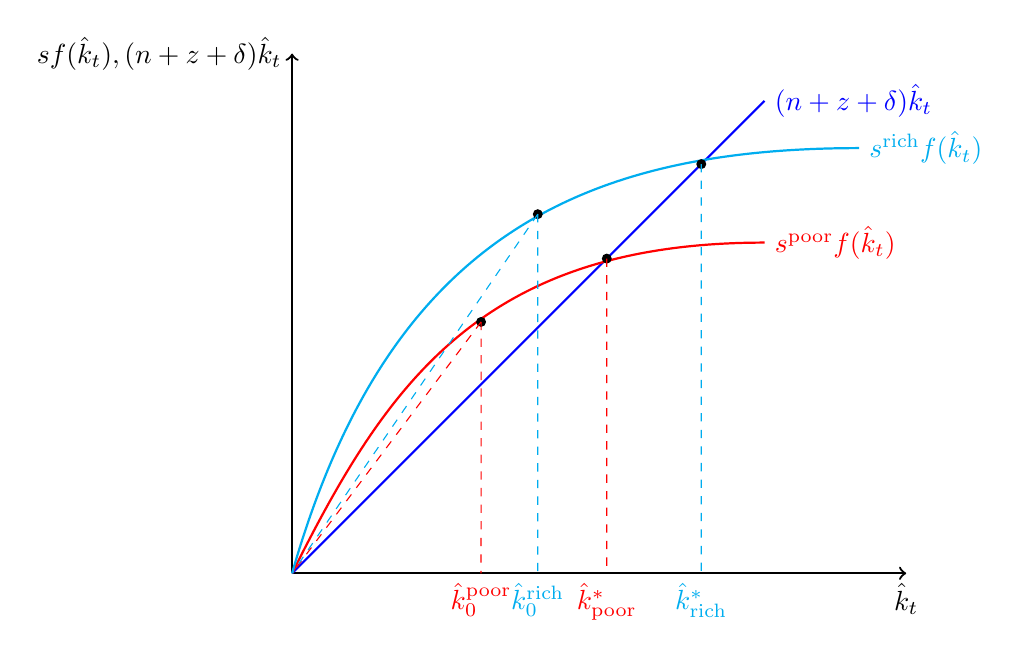
\begin{tikzpicture}[scale=1.2, domain=0:6]
  % Axes
  \draw[thick, ->] (0,0) node[below left] {} -- (6.5,0) node[below] {$\hat{k}_{t}$};
  \draw[thick, ->] (0,0) -- (0,5.5) node[left] {$sf(\hat{k}_{t}), (n+z+\delta)\hat{k}_{t}$};

  % Depreciation line ( \delta k )
  \draw[thick, blue] (0,0) -- (5,5) node[right] {$(n+z+\delta)\hat{k}_{t}$};

  % Saving curve ( sf(k) )
  \draw[thick, red] (0,0) .. controls (1,2) and (2,3.5) .. (5,3.5) node[right] {$s^\text{poor}f(\hat{k}_{t})$};

  % Saving curve ( sf(k) )
  \draw[thick, cyan] (0,0) .. controls (1,3.5) and (3,4.5) .. (6,4.5) node[right] {$s^\text{rich}f(\hat{k}_{t})$};

  % Steady state markers
  \coordinate (poorss) at (3.33, 3.33);
  \fill[black] (poorss) circle (1.5pt);
  \coordinate (richss) at (4.33, 4.33);
  \fill[black] (richss) circle (1.5pt);
  \coordinate (rich) at (2.6, 3.8);
  \fill[black] (rich) circle (1.5pt);
  \coordinate (poor) at (2, 2.66);
  \fill[black] (poor) circle (1.5pt);
  \draw[red, dashed] (poorss) -- (3.33,0) node[below] {$\hat{k}^*_\text{poor}$};
  \draw[cyan, dashed] (richss) -- (4.33,0) node[below] {$\hat{k}^*_\text{rich}$};
  \draw[red, dashed] (poor) -- (2,0) node[below] {$\hat{k}^\text{poor}_0$};
  \draw[cyan, dashed] (rich) -- (2.6,0) node[below] {$\hat{k}^\text{rich}_0$};
  \draw[red, dashed] (poor) -- (0,0);
  \draw[cyan, dashed] (rich) -- (0,0);
\end{tikzpicture}

\end{document}